\section{Itération n°2}
\subsection{Objectif de l'itération}

Dans cette nouvelle itération, nous allons devoir coder des émetteurs et un récepteur afin de convertir le signal logique en un signal "analogique" NRZ (non-retour à zéro), RZ (retour à zéro) et NRZT. Le rôle du récepteur sera de convertir n'importe quel signal analogique en un signal logique. Pour se faire, nous allons donc devoir modifier notre code afin de répondre aux exigences.

\begin{figure}[H]
    \centering
    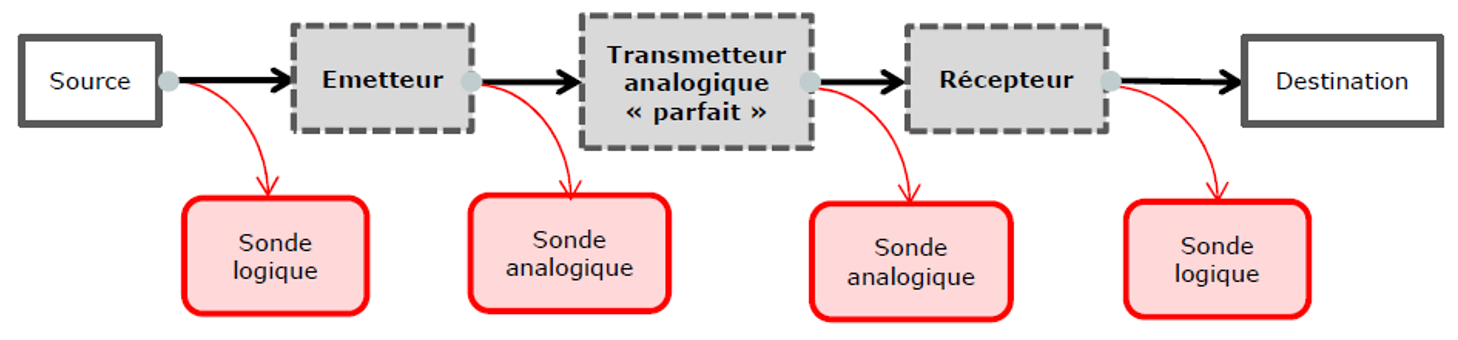
\includegraphics[width=1\textwidth]{image 5.png}
    \caption{\label{fig:image5}Chaîne de transmission itération n°2.}
\end{figure}

Un signal RZ signifie que le signal sera à l'état haut lorsque des 1 logiques seront transmis et à l'état bas lorsqu'il s'agit de 0 logique pendant la première demi-période. Il y a un retour à 0 à la deuxième demi-période du symbole (figure de gauche). Cependant dans ce projet, nous partirons du principe que l'émission à $V_{max}$ ou $V_{min}$ se situe entre le 1er et le 3ème tiers de la période symbole (figure de droite).

\begin{figure}[H]
    \centering
    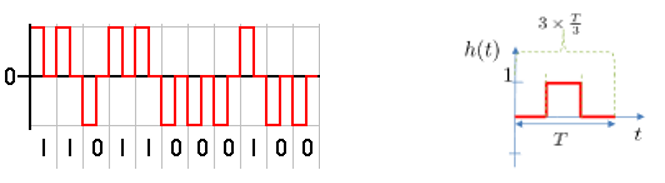
\includegraphics[width=1\textwidth]{image 6.png}
    \caption{\label{fig:image6}Schémas explicatifs signal RZ.}
\end{figure}

Un signal NRZ signifie que le signal sera à l'état haut lorsque des 1 logiques seront transmis et à l'état bas lorsqu'il s'agit de 0 logique. Contrairement au RZ, l'état est le même pendant toute la durée du temps symbole et d'utiliser trois fois moins de bande passante dans notre cas.

\begin{figure}[H]
    \centering
    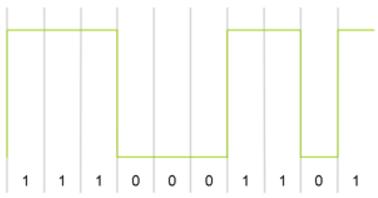
\includegraphics[width=0.5\textwidth]{image 7.png}
    \caption{\label{fig:image7}Schéma explicatif signal NRZ.}
\end{figure}

Un signal NRZT possède les mêmes propriétés qu'un signal NRZ. Cependant pour simuler le temps de montés des composants, chaque changement d'état sera représenté par une monté et descente progressive symbolisé sur $\frac{1}{3}$ des périodes symboles.

\begin{figure}[H]
    \centering
    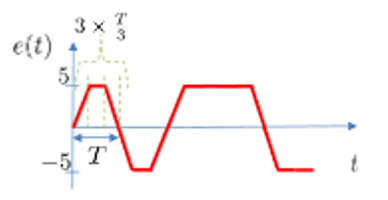
\includegraphics[width=0.5\textwidth]{image 8.png}
    \caption{\label{fig:image8}Schéma explicatif signal NRZT.}
\end{figure}

\textcolor{red}{Le cahier des charges nous donne des amplitudes maximum et minimum à respecter. Pour le codage NZR et NRZT, il faut que $V_{max} >= 0$ et $V_{min} >= 0$ et $V_{max} > V_{min} $
Pour le signal RZ, il faut que $V_{max} >= 0$ et $V_{min} = 0$ et $V_{max} > V_{min} $ }

\subsection{Organisation}

Pour nous permettre de répondre aux demandes de l'itération (mise en place d'une transmission analogique), nous allons devoir créer deux nouveaux éléments par rapport au code de la première itération. Ces modifications devront nous aider à lancer le programme tout en prenant en compte les paramètres d'entrée que nous rentrerons dans le terminal.
Nous ne devrions plus avoir d'erreurs sur notre code et ne pas avoir d'erreurs sur les signaux émis et reçus. Pour vérifier cela, nous utiliserons le calcul du TEB et afficherons les graphiques permettant de comparer à vue d'œil les éventuelles erreurs et leur emplacement.
Avant de commencer à développer notre code nous avons utilisé l'application "Project" d'Office 365 afin de nous permettre de créer un diagramme de Gant. Ce diagramme nous permet de classer les actions à faire (par catégories, par acteurs, par priorité) et de mettre des échéances afin de respecter les délais. Vous trouverez ci-dessous un exemple de diagramme Gant que nous avons fait pour cette seconde itération :

\begin{figure}[H]
    \centering
    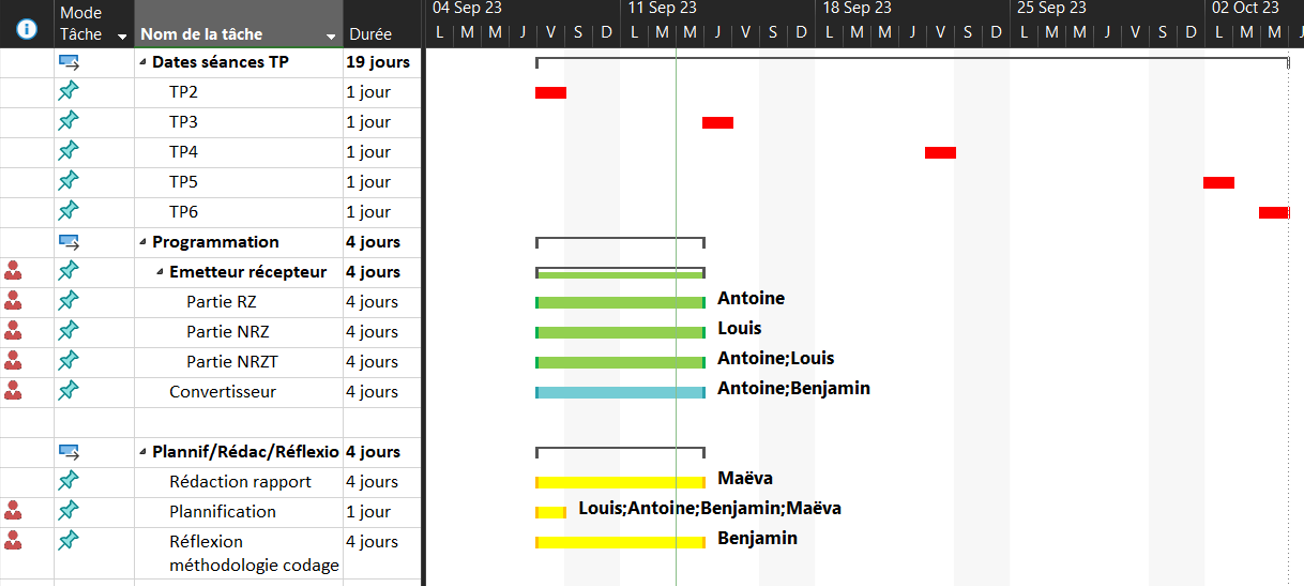
\includegraphics[width=1\textwidth]{image 9.png}
    \caption{\label{fig:image9}Diagramme de Gant itération 2.}
\end{figure}

Pour le développement de notre code, nous allons utiliser l'application Intellij Idea nous permettant de partager plus facilement les codes que nous déposons sur le projet que nous avons créé sur GitLab. La combinaison des 2 nous permet de modifier le code tous en même temps sans empiéter sur les modifications des-uns et des-autres. Intellij Idea nous permet également de créer des branches et de ne commit sur une interface graphique. Il est donc important de se répartir les tâches, ce que nous avons fait dans le diagramme de Gant.

\subsection{Procédures de développement}
\subsubsection{Emetteur}

L'émetteur à un rôle important. Il permet de convertir un signal logique en signal pseudo-analogique. Trois codages en ligne sont attendus pour ce projet. La logique qui repose sur ceux-ci sont la même. On prend le signal logique en entrée, puis en fonction de son état (0 ou 1), on le transforme en une série de flottant qui sera adapté au codage en ligne souhaité. Le nombre d'échantillonnage par symbole sera un paramètre à choisir lors des lancements de simulations (nommé nb\_samples par la suite) ainsi que l'amplitude maximum ($V_{max}$) et minimum ($V_{min}$).

\textbf{Emetteur NRZ :}

Il s'agit de l'émetteur le plus simple à coder. On prend le symbole logique en entrée et s'il s'agit d'un état à 1, alors on émet un nombre de flottant égale à nb\_samples ayant pour amplitude $V_max$. Pour l'état à 0, on émet le même nombre de flottant mais ayant pour amplitude $V_{min}$.

\begin{figure}[H]
    \centering
    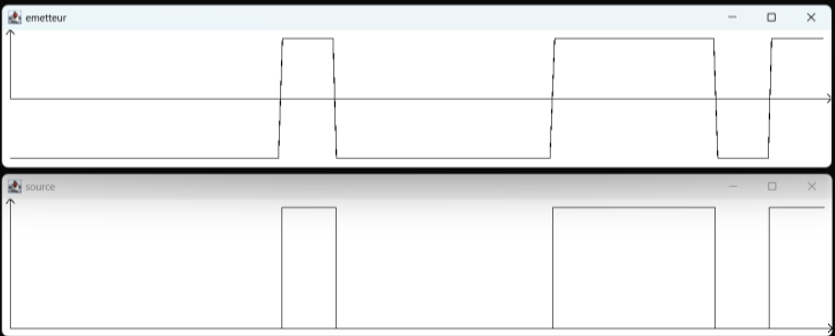
\includegraphics[width=1\textwidth]{image 10.png}
    \caption{\label{fig:image10}Sortie de la source et de l'émetteur NRZ.}
\end{figure}

Ci-dessus le graphique en sortie de la source et de l'émetteur NRZ. On retrouve bien une amplitude égale à $V_{max}$ pendant une durée symbole pour un état logique 1 et une amplitude égale à $V_{min}$ pendant une durée symbole pour un état logique à 0.

Emetteur RZ :

L'émetteur RZ est légèrement plus compliqué que le signal NRZ. La construction d'un symbole se passe en trois étapes.

\begin{itemize}
    \item Sur le premier tiers $(\frac{nb\_samples}{3})$, les flottants ont pour amplitude 0.
    \item Sur le deuxième tiers $(]\frac{nb\_samples}{3}$,$\frac{nb\_samples}{3}*2])$, les flottants ont pour valeur $V_{max}$ si le bit d'état logique est à 1 et $V_{min}$ si le bit est à 0.
    \item Sur ce dernier tiers, les flottants ont de nouveau une amplitude de 0.
\end{itemize}

\begin{figure}[H]
    \centering
    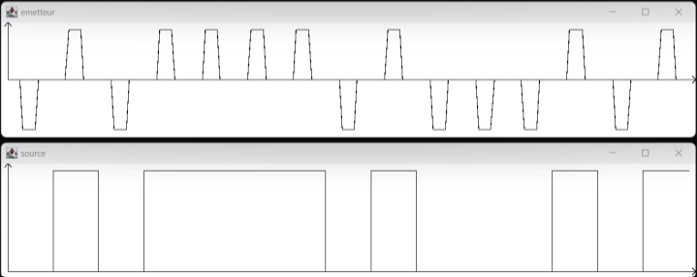
\includegraphics[width=1\textwidth]{image 11.png}
    \caption{\label{fig:image11}Sortie de la source et de l'émetteur RZ.}
\end{figure}

Ci-dessus le graphique en sortie de la source et de l'émetteur RZ. On apercevoir qu'un symbole logique est représenté par un symbole analogique composé en trois parties : le premier et dernier tiers à 0 et le deuxième tiers avec une amplitude à $V_{max}$ ou $V_{min}$.

\textbf{Emetteur NRZT :}

C'est le transmetteur le plus complexe à faire. Il reprend les caractéristiques du NRZ mais possède une pente montante et descendante au 1er et dernier tiers. Avant toute chose, il faut calculer un pas qui sera utilisé pour la pente. Pour cela, on utilise cette formule : $ pas = \frac{Vx}{\frac{nb\_samples}{3}} $ avec $V_x$ ayant $V_{max}$ ou $V_{min}$ en fonction du bit logique.

La construction d'un sylmbole se passe en trois étapes :
\begin{itemize}
    \item Sur le premier tiers $ \left(\frac{nb\_samples}{3} \right) $, les flottants ont une amplitude déterminée par le pas pour construire une rampe vers $V_x$.
    \item Sur le deuxième tiers $(]\frac{nb\_samples}{3}, \frac{nb\_samples}{3}*2]) $, les flottants ont pour valeur $V_{max}$ si le bit d'état logique est à 1 et $V_{min}$ si le bit est à 0.
    \item Sur le dernier tiers, les flottants ont une amplitude déterminée par le pas pour construire une rampe vers 0. Néanmoins, si plusieurs bits logiques de même signe se suivent, il n'y a pas de rampe entre le premier et le dernier tiers des bits analogiques correspondants. On reste sur une amplitude $V_{max}$ et $V_{min}$.
\end{itemize}

\begin{figure}[H]
    \centering
    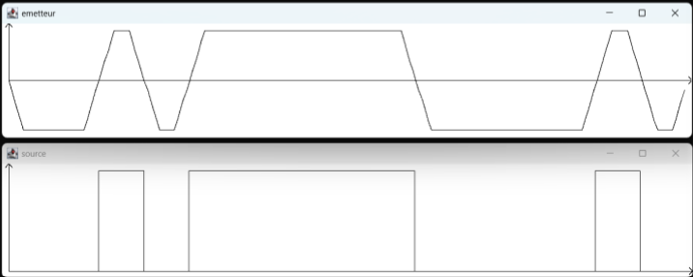
\includegraphics[width=1\textwidth]{image 12.png}
    \caption{\label{fig:image12}Sortie de la source et de l'émetteur NRZT.}
\end{figure}

Ci-dessus le graphique en sortie de la source et de l'émetteur NRZT. On remarque que le signal en sortie d'émetteur correspond bien à la description faite précédemment. On observe bien les pentes vers $V_x$ et 0 mais également la conservation de l'amplitude $V_x$ lorsque plusieurs bits logiques se suivent.

\subsubsection{Récepteur}

Le récepteur à un enjeu primordial, il est capable de recevoir un signal analogique et de le convertir en un signal logique (même type que le signal source). Notre exigence était d'avoir un seul récepteur qui puisse traiter n'importe quel signal analogique.
Pour ce faire, on utilise comme méthode de moyenner les valeurs reçues sur la durée d'un temps symbole. Préalablement, nous avons déterminer un seuil de décision qui correspond à $\frac{V_{max} + V_{min}}{2}$.
Il peut ainsi fluctuer en fonction des valeurs seuil choisi. Si la moyenne se situe au-dessus du seuil de décision, alors le bit d'état logique sera à 1. Si la moyenne se situe en-dessous du seuil de décision, alors le bit d'état logique sera à 0.

\subsection{Tests}

Par manque de temps, nous n'avons pas réalisé de test à proprement parler pour tester chaque ligne des nouvelles classes de l'itération. Nous avons seulement effectué un contrôle visuel grâce aux sondes placées aux différents endroits. Le principal contrôle étant de s'assurer que le signal reçu est le même que le signal émis comme il s'agit d'un canal parfait.
Pour les prochaines itérations, nous effectuerons de vrai test avec notamment des outils pour tester la couverture de ceux-ci.

\subsection{Performances}

Nous sommes toujours dans le cas d'un canal de transmission parfait. Que ce soit avec n'importe quel codage de signal, nous arrivons à retrouver les bits émis par la source.

Voici la simulation pour un signal généré grâce à une source aléatoire puis encodé en NRZ :

\begin{figure}[H]
    \centering
    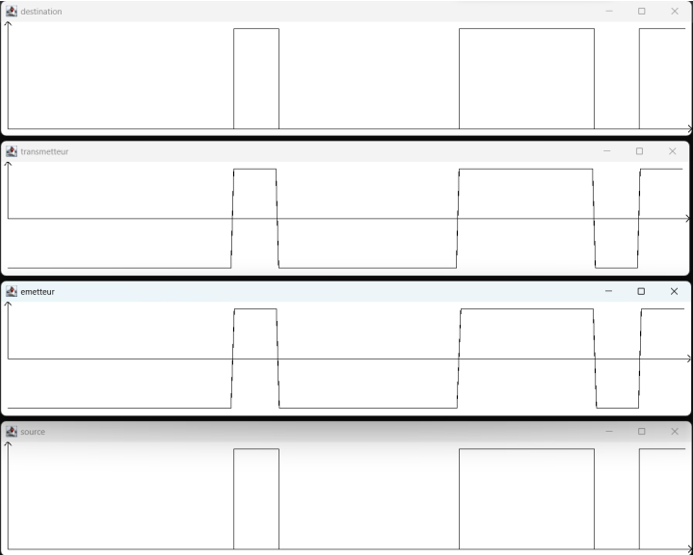
\includegraphics[width=1\textwidth]{image 13.png}
    \caption{\label{fig:image13}Simulation d'un signal généré puis encodé en NRZ.}
\end{figure}

Voici la simulation pour un signal généré grâce à une source aléatoire puis encodé en RZ :

\begin{figure}[H]
    \centering
    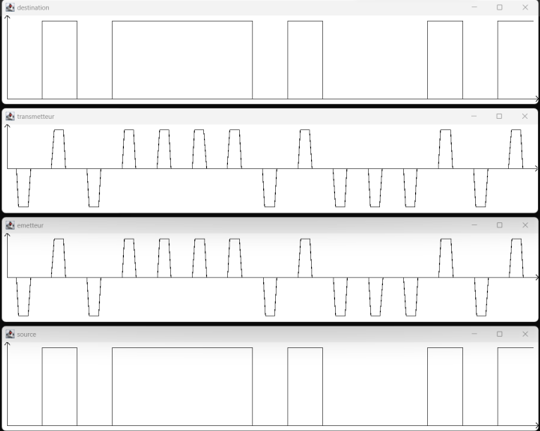
\includegraphics[width=1\textwidth]{image 14.png}
    \caption{\label{fig:image14}Simulation d'un signal généré puis encodé en RZ.}
\end{figure}

Voici la simulation pour un signal généré grâce à une source aléatoire puis encodé en NRZT :

\begin{figure}[H]
    \centering
    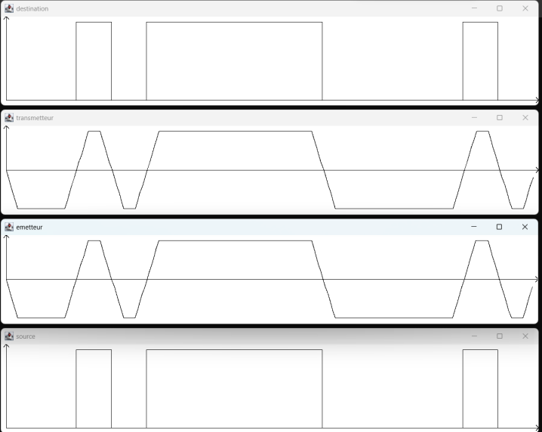
\includegraphics[width=1\textwidth]{image 15.png}
    \caption{\label{fig:image15}Simulation d'un signal généré puis encodé en NRZT.}
\end{figure}

Nous observons que la sortie du transmetteur est purement identique à la source. C'est normal car il s'agit d'un canal parfait. Le TEB est donc de 0. Le codage en ligne, quel qui soit, n'a pas d'impact
lorsqu'il est émis sur un transmetteur parfait.

\subsection{Conclusion}

Notre projet évolue. Lors de la première itération, notre chaine de transmission était opérationnelle avec comme fonctionnalités le type de source et l'observation de la sortie du canal.
Maintenant, nous sommes capables de convertir le signal de la source en un codage en ligne (RZ,NRZ et NRZT) et d'effectuer la manœuvre inverse en bout de canal afin de retrouver le signal de départ.

Nous avons également eu un problème de gestion du temps (mauvaise compréhension de la date de dépôt). Cette erreur ne nous a pas permis de livrer l'itération avec l'ensemble des attentes (tests, scripts). Ce manque sera comblé lors de la prochaine itération.
\textcolor{red}{Suite aux complications que nous avions eu lors de la seconde itération, nous avons profité de la troisième pour corriger nos erreurs et mettre à jour le code. Nous avons donc modifié le code du côté de l'emetteur pour le RZ afin que ce dernier fonctionne. Nous avons également modifié les codes du côté de l'émetteur et du récepteur pour le NRZT. Grâce à ces modifications nous n'avons plus de décalage lors de la simulation des signaux RZ et NRZT.}

Lors de la prochaine étape, il faudra créer un nouveau transmetteur afin d'avoir une transmission non-idéale avec canal bruité de type "gaussien".